\documentclass[12pt]{article}

\usepackage{sbc-template}

\usepackage{graphicx,url}
\usepackage{csvsimple}
\usepackage{subfigure}

\usepackage{amssymb}% http://ctan.org/pkg/amssymb
\usepackage{pifont}% http://ctan.org/pkg/pifont
\newcommand{\cmark}{\ding{51}}%
\newcommand{\xmark}{\ding{55}}%

\usepackage{multirow}
\usepackage[brazil]{babel}    
\usepackage[utf8]{inputenc}
 
\sloppy

\title{Reprodução de um elemento de artigo}

\author{Gustavo Ciotto Pinton\inst{1} }


\address{Instituto de Computação -- Universidade Estadual de Campinas
(UNICAMP)\\
  Av. Albert Einstein, 1251, Cidade Universitária, Campinas/SP \\
  Brasil, CEP 13083-852, Fone: [19] 3521-5838
  \email{ra117136@unicamp.br}
}

\begin{document} 

\maketitle

\begin{abstract}
This report describes the curves \textbf{single thread} and \textbf{ideal} from
figure 3 in the article Accelerating Decoupled Look-ahead via Weak Dependence
Removal: A Metaheuristic Approach \cite{artigo}. We used
Sniper micro-architecture simulator and pinballs of SPEC CPU2006 benchmarks with
1 billion instruction detailed regions and no warm up. We compared the effects
of ideal caches and branch predictors on IPC measures. A gshare predictor was
implemented and added to the simulator. Some difficulties met during the project
will be also described.
\end{abstract}
     
\begin{resumo} 
Este relatório reproduz as curvas \textbf{single thread} e \textbf{ideal}
contidos na figura 3 do artigo Accelerating Decoupled Look-ahead via Weak Dependence Removal: A Metaheuristic
Approach \cite{artigo}. Foi utilizado o simulador de micro-arquiteturas Sniper e
os pinballs dos benchmarks do SPEC CPU 2006 com regiões detalhadas contendo 1
bilhão de instruções e sem quaisquer intruções de warmup. Comparou-se os efeitos
de caches e preditores ideais no IPC. Um preditor gshare foi implementado para o
simulador. Serão discutidos também algumas dificuldades encontradas durante o
projeto.
\end{resumo}


\section{Introdução}

O artigo escolhido para este projeto foi \textit{Accelerating Decoupled
Look-ahead via Weak Dependence Removal: A Metaheuristic Approach} \cite{artigo},
cujo objetivo foi propor um método para melhorar o desempenho de \textit{look
ahead threads} a partir de algoritmos genéticos. Neste artigo, os autores
argumentam que o IPC de uma aplicação com apenas uma \textit{thread} é limitado
justamente pelo IPC desta \textit{thread} auxiliar, que é executada em um
outro \textit{core}.

A ideia principal deste tipo de arquitetura é gerar uma versão reduzida da
programa principal, de maneira a não obter um grande \textit{overhead} e
redundância (executar o mesmo programa duas vezes), e a diminuir os efeitos
causados por \textit{misses} nos \textit{caches} e nos preditores de salto, à
medida que evita a perda de ciclos em casos em que o preditor previu
erroneamente o salto ou quando o dado procurado não se encontra no primeiros
níveis de \textit{cache}. Tal versão reduzida é executada, conforme já dito no
parágrafo anterior, em outro \textit{core} do processador, paralelamente à
\textit{thread} principal. O desafio reside, portanto, em como obter uma
\textit{lookup thread} representativa, mas, ao mesmo tempo, a mais simples
possível, já que, de acordo com \cite{artigo}, tal \textit{thread} torna-se o
novo limite de velocidade do sistema.

Nestes sistemas, um \textit{parser} é utilizado para analisar o binário do
programa e criar uma versão \textit{esqueleto}, que consistirá na
\textit{lookup thread}. Durante a execução, esta \textit{thread} envia os
resultados de saltos condicionais já comitados através de uma fila para o
\textit{core} principal, que, por sua vez, pode utilizar tais resultados no seu
processamento. Além disso, dados são diretamente enviados ao \textit{caches}
compartilhados. Os autores destacam a existência de \textit{dependências
fracas}, isto é, instruções que contribuem o mínimo para os propósitos da
\textit{lookup ahead thread}. Exemplos destes tipos de instruções podem ser
instruções aritméticas e lógicas que não mudam o resultado de um registrador na
maior parte do tempo, ajustes inúteis em registradores (realizar uma operação em
um registrador sendo que ele será o alvo de um \textit{store} em seguida) e
instruções de \textit{store}/\textit{load} que sempre escrevem ou carregam o
mesmo valor. Infelizmente, sua análise torna-se muito difícil caso seja
realizada estaticamente, uma vez que uma instrução se torna uma dependência
fraca de acordo com o contexto do programa. Os autores ainda afirmam que não
conseguiram encontrar nenhuma característica especial em comum que pudesse
identificá-las rapidamente no momento de geração dos esqueletos. É importante
lembrar que a identificação de uma instrução errada pode, de fato, piorar o
desempenho do sistema, dado que novos \textit{misses}, que não ocorreriam
naturalmente, podem ser inseridos.

Sendo assim, dada a natureza dinâmica das dependências, a não-linearidade dos
efeitos de performance e a interdependência das cadeias de instruções, a melhor
solução encontrada pelos autores foi recorrer a heurísticas e análise de código
para predizer a fraca dependência. No caso, eles utilizaram algoritmos genéticos
e propuseram um novo método para encontrar instruções com grande probabilidade de
serem fracas dependências. O método proposto foi capaz de aumentar a performance
total dos sistemas testados em até 1.48x (1.14x média geométrica).

Apesar de toda a explicação, os elementos da figura escolhida para a reprodução
não abrangem diretamente as ideias anteriores. O objetivo neste relatório é
replicar as curvas \textit{ideal} e \textit{single thread} da figura
\ref{fig:artigo} (figura 3 de \cite{artigo}, página 3). A curva relativa a
\textit{single thread} corresponde à execução \textit{normal} dos
\textit{benchmarks}, enquanto que a \textit{ideal} supõe que nunca ocorrerão
\textit{mispredictions} nos preditores ou \textit{cache misses}, ou seja,
supõe-se que todos os dados estão disponíveis nos \textit{caches} e que o
preditor sempre acertará suas previsões.
As duas outras curvas, por exigirem uma grande alteração na estrutura dos
simuladores, serão deixadas para uma outra oportunidade. Destaca-se, ainda, que
os autores utilizaram os \textit{benchmarks} do \texttt{SPEC CPU2000}. Por
dificuldades de licença e por razões de simplicidade (já possuímos os
\textit{pinballs}), usamos o \texttt{SPEC CPU2006}. 

\begin{figure}[h!]
  \centering
  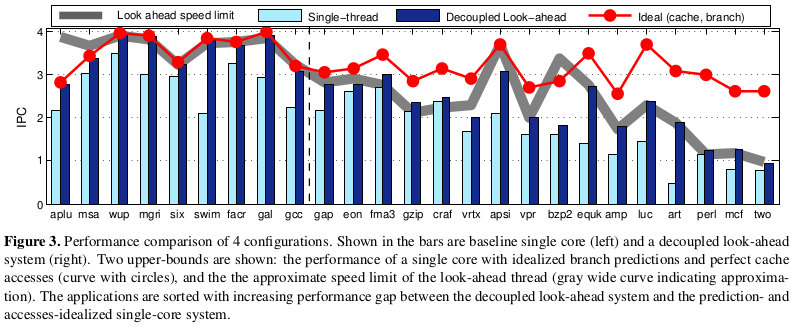
\includegraphics[width=\textwidth]{img/fig3}%
  \label{fig:artigo}%
  \caption{Figura escolhida para reprodução com legenda original. Extraída de
  \cite{artigo}.}
\end{figure}

Em um primeiro contato com os autores, fui aconselhado a utilizar o
\textit{gem5} ou o \textit{SimpleScalar} como simuladores. Entretanto,
escolhemos o \textit{sniper}, dado experiências anteriores com
a ferramenta \textit{pin}, no qual tal simulador é baseado. O \textit{sniper}
implementa o modelo de processamento chamado \textit{interval core model}, que
aumenta o grau de abstração da simulação, permitindo tempos menores de avaliação
e desenvolvimento \cite{sniper}. Contrariamente ao \textit{gem5}, por exemplo, que
modela todos os estágios de \textit{pipeline}, o \textit{sniper} divide a
execução em intervalos, delimitados pelos eventos denominados de \textit{miss
events}, tais como \textit{branch mispredictions}, \textit{cache} e TLB
\textit{misses}, etc. O simulador mantém um registro interno do tempo de
simulação em cada \textit{core} e, a cada \textit{miss event}, esse contador é
aumentado com o tempo do respectivo evento. Dessa forma, o \textit{sniper} é
capaz de calcular uma série de estátisticas, como o IPC, que foi utilizado
neste relatório como métrica.

Enfim, neste relatório serão apresentados os resultados das curvas
\textit{ideal} e \textit{single thread} da figura \ref{fig:artigo} para a
configuração do artigo (consultar próximas seções) e para uma configuração
padrão do \textit{sniper}, que modela a microarquitetura \textit{Gainestown} da
\textit{Intel}.

\section {Implementação}

Nesta seção, serão discutidos detalhes da implementação e algumas dificuldades
encontradas na configuração e instalação do \textit{sniper}.

\subsection{Configuração do \textit{sniper}}

O \textit{sniper} foi executado em uma máquina virtual de 64 \textit{bits
Ubuntu 14.04 LTS} e foi compilado com o \textit{gcc 4.4}. A compilação não
apresentou nenhuma grande dificuldade em específico, diferentemente da execução
dos \textit{pinballs}, que exigiu um pouco mais de estudo da ferramenta. Dois
tipos de \textit{pinballs} foram utilizados: aqueles com 100M instruções de
\textit{warmup} e 30M instruções na região detalhada, e, posteriormente, os de
1B de instruções na região detalhada e sem \textit{warmup}. Para os últimos, a
integração com o \textit{sniper} foi bem simples, visto que foi necessário
apenas o uso da opção \texttt{--pinballs} na comando \texttt{run-sniper}. Para
os primeiros, entretanto, o desafio foi dizer ao simulador para executar a
região de \textit{warm up} no modo correto, isto é, \texttt{CACHE\_ONLY}. As
seguintes propostas foram implementadas:

\begin {itemize}
	\item Utilizar a opção \texttt{--roi}: o uso dessa opção fazia com que todo o
	\textit{pinball} fosse executado em modo \texttt{CACHE\_ONLY}, gerando nenhum
	arquivo de saída e nenhuma estatística.
	\item Implementação de \textit{pintool}: uma nova \textit{pin tool} foi
	implementada a fim de contar as instruções e chamar a função
	\texttt{SimRoiStart()} explicitamente. Essa função e várias outras são
	fornecidas pelo arquivo \path{sniper/include/sim_api.h} e podem ser adicionadas
	aos programas simulados. Infelizmente, o \textit{sniper} não é capaz de
	executar o binário do \textit{pin}, uma vez que este último foi pré-compilado
	em uma máquina de 32 \textit{bits}.
	\item Uso de uma máquina virtual de 32 \textit{bits}: já que o \textit{pin} não
	pode ser rodado na compilação em máquinas de 64 \textit{bits}, compilei o
	\textit{sniper} novamente, mas agora em uma máquina virtual de 32
	\textit{bits}. Nesta oportunidade, não pude executar corretamente, uma vez que
	o \textit{pinballs} haviam sido criados em máquinas de 64 \textit{bits} e não
	poderiam rodar em máquinas de 32 \textit{bits}.
	\item Utilizar um \textit{script python} com a opção \texttt{-s}: depois de
	perguntar no \textit{Google group} do simulador, recebi a resposta de que um
	\textit{script python} capaz de contar as instruções é disponível no diretório
	\texttt{sniper/scripts}. Tal \textit{script} se chama \texttt{roi-icount.py} e,
	no nosso caso, deve ser chamado com o parâmetro 0:100000000:30000000, indicando
	a largura de instruções de cada região.
\end{itemize}

Apesar de todo o trabalho de configuração para o uso dos \textit{pinballs} com
100M de instruções de \textit{warm up}, eles não foram utilizados, uma vez que
os resultados encontrados foram muito distantes daqueles encontrados no artigo.
Ao invés deles, usamos os \textit{pinballs} com 1B de instruções na região
de interesse. Maiores detalhes podem ser encontrados na seção
\textbf{Resultados}.

\subsection{Ambiente de testes do artigo}

A tabela \ref{tab:ambiente} resume a configuração em que os resultados do artigo
foram encontrados. As linhas indicadas por um \cmark ~puderam ser corretamente
configuradas no \textit{sniper}, enquanto que as indicadas por um \xmark ~não
puderam ser atribuídas, uma vez que modificações mais profundas no modelo de
intervalos, comentado na seção \textbf{Introdução}, deveriam ser realizadas.
Dado o prazo e os problemas enfrentados durante o projeto, preferimos deixar tais requisitos
para o projeto 4.

\begin{table}[h]
    \centering
	\caption{\label{tab:ambiente} Configuração utilizada no artigo. Extraído de
	\cite{artigo}.}
	\begin{tabular}{| l | l | l | }
		\hline
		\multicolumn{3}{|c|}{ \textbf{Baseline core}} \\ \hline
		Fetch/Decode/Issue/Commit & 8/4/6/6 & \xmark\\ 
		ROB & 128 & \cmark \\ 
		Functional units & INT 2+1 mul +1 div, FP 2+1 mul +1 div & \xmark\\
		Fetch Q/ Issue Q / Reg. (int,fp) & (32, 32) / (32, 32) / (80, 80) & \xmark\\ 
		LSQ(LQ,SQ) & 64 (32,32) 2 search ports & \xmark\\
		Branch predictor & Gshare – 8K entries, 13 bit history & \cmark \\ 
		Br. mispred. penalty & at least 7 cycles & \cmark \\ 
		L1 data cache (private) & 32KB, 4-way, 64B line, 2 cycles, 2 ports &
		\cmark \\
		L1 inst cache (private) & 64KB, 2-way, 128B, 2 cycles & \cmark \\ 
		L2 cache (shared) & 1MB, 8-way, 128B, 15 cycles & \cmark \\ 
		Memory access latency & 200 cycles & \cmark \\ \hline
		
	\end{tabular}
\end{table}

As configurações da tabela \ref{tab:ambiente} podem ser encontradas no arquivo
\path{article.cfg}. Para o caso ideal, utilizamos o arquivo
\path{ideal-article.cfg}, que extende o primeiro, mas modifica algumas
propriedades de forma a obter o valor máximo de IPC. Para o preditor ideal,
mudamos a propriedade \texttt{mispredict\_penalty} para 0 e para todos os
\textit{caches}, a propriedade \texttt{perfect} para \texttt{true}. O ajuste da
latência da memória, por sua vez, é realizado pelo parâmetro
\texttt{perf\_model/dram/latency}. O ajuste do tamanho do \textit{reorder
buffer} é feito por \texttt{window\_size}, já que o simulador
mantém uma janela de instruções para cada \textit{core} simulado
\cite{interval}, o que equivale justamente à função do \textit{reorder buffer}
em um processador super-escalar \textit{out-of-order}. Além disso, implementamos um
preditor do tipo \textit{gshare}, a partir das classes abstratas fornecidas
pelo simulador com as características apresentadas acima. Enfim, utilizamos o
modelo do processador padrão \textit{Nehalem} para modelar as instruções e
micro-instruções. Uma das metas do projeto 4 é implementar um modelo mais
parecido ao POWER5, que foi utilizado no artigo.

\subsection{Implementação de preditor \textit{Gshare}}

A implementação de um modelo de preditor no \textit{sniper} é realizado a partir
da definição de uma classe abstrata chamada \texttt{BranchPredictor}, que possui
2 métodos virtuais, sendo eles \texttt{predict()} e \texttt{update()}.
Todos recebem como parâmetro o endereço atual de \textit{PC}. O primeiro retorna
um valor \textit{booleano}, indicando se a operação de salto deve ou não ser
realizada e o segundo atualiza o estado do preditor e o histório de saltos de
acordo com o resultado do salto após que tal operação tenha sido
\textit{comitada}. Implementou-se, portanto, a classe
\texttt{GShareBranchPredictor} que redefine estes dois métodos e mantém uma
variável contendo o estado dos 13 últimos saltos (13 \textit{bits}). Tal classe
possui também um vetor de preditores que implementam a máquina de estados de 2
\textit{bits} (classe \texttt{SaturatingPredictor<2>}) e, a cada operação, o
índice desse vetor é obtido através de um \textit{ou exclusivo} entre o endereço
PC e a variável de histórico. Por fim, é necessário adicionar essa classe no
método \texttt{create()} do arquivo \path{branch_predictor.cc} e compilar o
\textit{sniper} novamente.

\section{Resultados}

Contrariamente aos resultados da figura \ref{fig:artigo} que foram obtidos para
os \textit{benchmarks} do \texttt{SPEC CPU2000}, os testes produzidos neste
relatório foram gerados a partir dos \textit{pinballs} do \texttt{SPEC CPU2006}. 

No total, 4 arquivos de configuração foram utilizados, dois para a
micro-arquitetura \textit{Gainestown} e duas para a micro-arquitetura do artigo.
É necessário observar que o caso referente ao \textit{Gainestown} não possui
alguma ligação com o artigo, porém ele foi executado mesmo assim com o intuito
de testar completamente o ambiente e de comparar os resultados finais. Conforme
comentado anteriormente, utilizamos os \textit{pinballs} com 1B de instruções na
região detalhada, gastando, em média, aproximadamente 30 minutos para cada
entrada dos \textit{benchmarks}.  A figura \ref{fig:gainestown} representa os
resultados para a micro-arquitetura \textit{Gainestown} e a \ref{fig:artigocfg},
para a configuração da tabela \ref{tab:ambiente}. Os \textit{benchmarks} foram
posicionados em ordem crescente de diferença entre o desempenho ideal e o
normal.

Observa-se que os desempenhos ideais das duas execuções apresentam IPCs 
muito parecidos entre si, valendo 1.93 e 1.68 em média geométrica para a
configuração do artigo e \textit{Gainestown}, respectivamente. As medidas de IPC
para os casos normais variam mais entre si em média geométrica, valendo de 0.65
para a configuração do artigo e 1.09 para o \textit{Gainestown} (variação de
1.68x).
 
\begin{figure}[ht]
  \centering
  \subfigure[Resultados da simulação dos \textit{benchmarks} do \texttt{SPEC
  2006} para o arquivo de configuração \textit{Gainestown}.]{%
    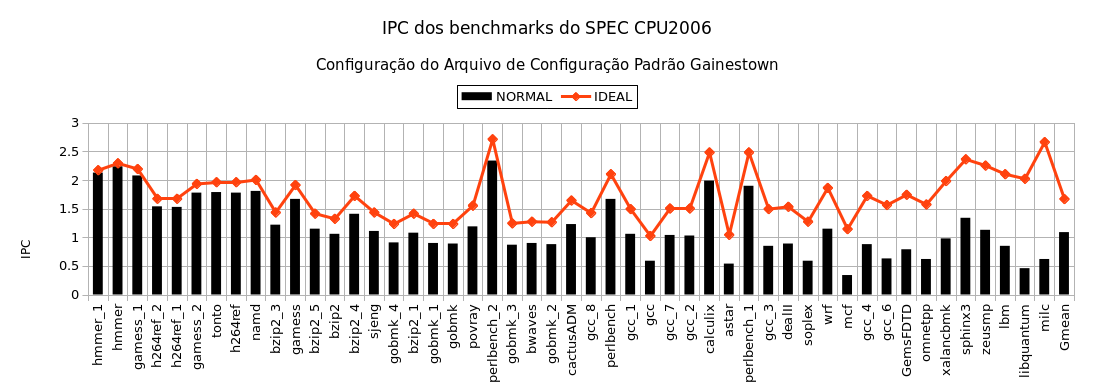
\includegraphics[width=\textwidth]{img/gainestown}%
    \label{fig:gainestown}%
  }
  
  
  \subfigure[Resultados da simulação dos \textit{benchmarks} do \texttt{SPEC
  2006} para o arquivo de configuração do artigo.]{%
    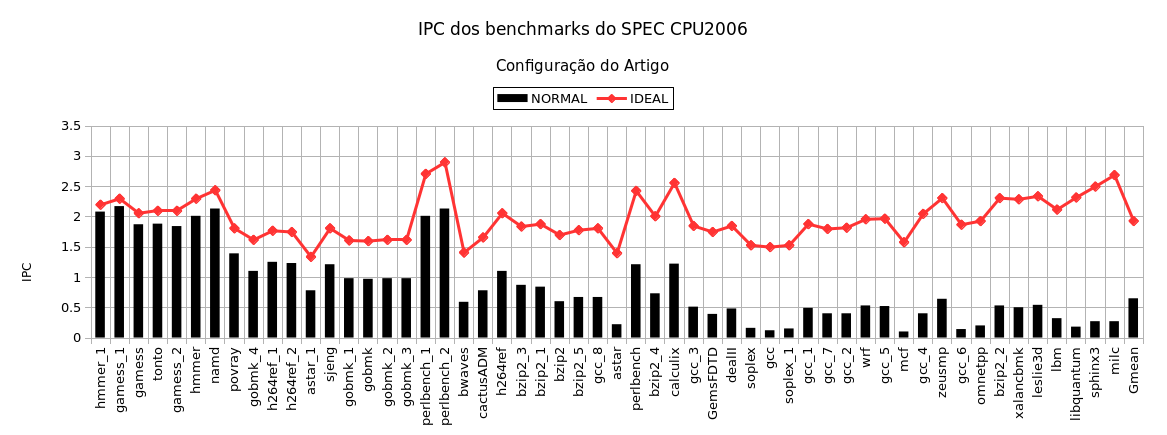
\includegraphics[width=\textwidth]{img/article}%
    \label{fig:artigocfg}%
  }
  \caption{Resultados da simulação.}
\end{figure}

Em relação aos resultados encontrados no artigo, nota-se que, em geral, eles são
maiores que os encontrados nos experimentos encontrados neste relatório. Uma
possível explicação reside no fato de que os testes produzidos em \cite{artigo}
utilizaram os programas completos para as estatísticas. Durante os testes com os
\textit{pinballs} com 130M de instruções, constatou-se que os resultados obtidos
eram muitos inferiores àqueles dos \textit{pinballs} de 1B instruções. É
evidente que quanto mais instruções executarmos, mais parecidos serão os
resultados encontrados. Entretanto, o tempo de execução também cresce muito: se
assumirmos que o tempo de execução varia linearmente com o número de instruções,
a execução completa de um \textit{benchmark} com um 1 trilhão de instruções
levaria aproximadamente 500 horas!
  

\section{Conclusões}

Foi possível reproduzir, através do \textit{sniper}, resultados semelhantes
àqueles encontrados no artigo para as curvas \textit{ideal} e \textit{single
thread}, apesar de que diferentes \textit{benchmarks} foram utilizados. Duas
configurações foram testadas: uma para a microarquitetura \textit{Gainestown} e
a outra para o ambiente configurado no artigo. Notou-se que, em geral, a
primeira configuração apresentou resultados melhores de IPC, em média
geométrica. Implementou-se, ainda, um preditor to tipo \textit{gshare} a partir
das classes abstratas fornecidas pelo \textit{sniper}.


\bibliographystyle{sbc}
\bibliography{sbc-template}

\end{document}
